\documentclass[tikz,border=3mm, convert={outfile=mips32-decompiler.png}]{standalone}
\usepackage{tikz}
\usepackage{varwidth}
\usetikzlibrary{shapes.geometric,positioning}
\begin{document}

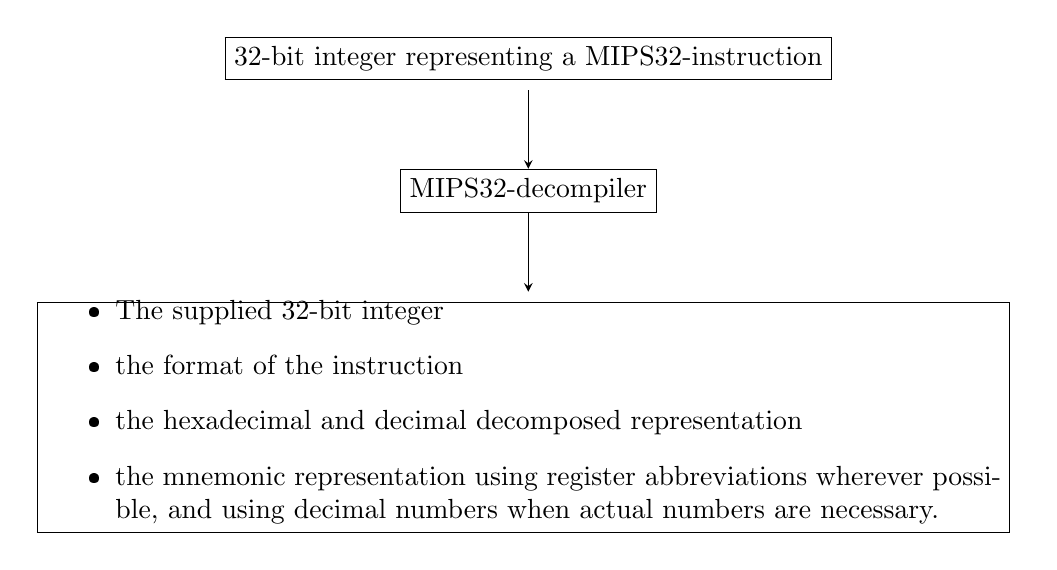
\begin{tikzpicture}[>=stealth]
  \node [draw] (decompiler) {MIPS32-decompiler};
  \node [above=of decompiler, align=center] (input) {\framebox{32-bit integer representing a MIPS32-instruction}};
  \node [below=of decompiler, align=center] (output) {
    \framebox{\begin{varwidth}{\linewidth}\begin{itemize}
          \item The supplied 32-bit integer
          \item the format of the instruction
          \item the hexadecimal and decimal decomposed representation
          \item the mnemonic representation using register
            abbreviations wherever possible, and using decimal numbers
            when actual numbers are necessary.
    \end{itemize}\end{varwidth}}
  };
  \draw [->] (input) -- (decompiler);
  \draw [->] (decompiler) -- (output);
\end{tikzpicture}
\end{document}
